\documentclass{article}
\usepackage{tikz}

\begin{document}

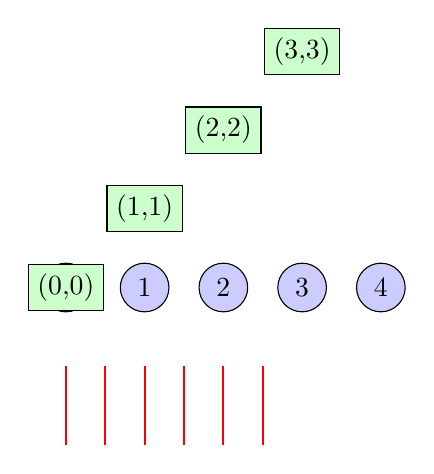
\begin{tikzpicture}
  % --- Simple foreach loop: draw circles along a line ---
  \foreach \x in {0,1,2,3,4} {
    \node[draw, circle, fill=blue!20] at (\x,0) {\x};
  }

  % --- Foreach with two variables ---
  \foreach \x/\y in {0/0, 1/1, 2/2, 3/3} {
    \node[draw, rectangle, fill=green!20] at (\x,\y) {(\x,\y)};
  }

  % --- Foreach with step size ---
  \foreach \x in {0,0.5,...,2.5} {
    \draw[red, thick] (\x,-1) -- (\x,-2);
  }
\end{tikzpicture}

\end{document}
